% !TEX root = ../lab2_report.tex
% ═══════════════════════════════════════════════════════════════
% 实验一：轴流压气机稳态特性试验
% ═══════════════════════════════════════════════════════════════

\section{实验一：轴流压气机稳态特性试验}

\subsection{实验目的}

\begin{enumerate}
    \item 掌握轴流压气机内流动、加功增压原理和稳态特性。
    \item 熟悉压气机气动参数测量和计算方法。
    \item 了解对转压气机的工作原理和性能特点。
\end{enumerate}

\subsection{实验原理}

研究两级低速轴流对转压气机的稳态特性。对转技术应用于航空发动机可以减小发动机轴向距离，同时降低发动机重量，提升增压能力。通过改变节流锥位置调节出口面积，测量不同转速下压气机的总压升和流量变化。压气机的等转速特性线反映了压气机在不同流量工况下的增压能力，是评估压气机性能的核心依据。

\subsection{实验装置}

实验采用两级低速轴流对转压气机，主要参数见表~\ref{tab:rotor_params}。进口为双扭线喇叭口，上下游转子分别由两个 7.5 kW 三相交流电机驱动，转速由变频器控制（0\textasciitilde3000 rpm），出口面积由节流锥控制。

\begin{table}[H]
\centering
\caption{对转压气机转子参数}
\label{tab:rotor_params}
\begin{tabular}{lcc}
\toprule
参数 & 上游转子 & 下游转子 \\
\midrule
最大转速 (rpm) & 3000 & 3000 \\
叶片数目 & 12 & 10 \\
叶尖弦长 (mm) & 95 & 95 \\
叶顶圆直径 (mm) & 501 & 501 \\
叶尖安装角 (°) & 26.9 & 21.6 \\
轮毂比 & 0.61 & 0.61 \\
旋向 & 顺时针 & 逆时针 \\
\bottomrule
\end{tabular}
\end{table}

\subsection{实验步骤}

\begin{enumerate}
    \item 启动稳态特性测量程序。
    \item 启动节流锥控制程序，将节流锥顶点移至出口截面。
    \item 零点采集：点击"系统操作→零点采集"，采集并存储零点。
    \item 点击"示波"按钮，开启前后变频器至目标频率。
    \item 依次测量各个工况点，每点待信号稳定后点击"采集"。
    \item 点击"结束存盘"保存数据。
    \item 重复以上步骤，分别测量其他转速下的特性。
    \item 实验结束：停止变频器，关闭测量程序和节流锥控制程序。
\end{enumerate}

\subsection{数据处理方法}

\subsubsection{质量流量计算}

进口截面直径 $D = 0.502$ m，流通面积
\begin{equation}
    A_{\text{inlet}} = \frac{\pi D^2}{4}
\end{equation}

空气密度由理想气体状态方程计算：
\begin{equation}
    \rho = \frac{P_{\text{atm}}}{R \cdot T_{\text{atm}}}, \quad R = 287.058\ \text{J/(kg·K)}
\end{equation}

进口速度由伯努利方程计算（不可压缩流动）：
\begin{equation}
    v = \sqrt{\frac{2(P_{\text{in}}^* - P_{\text{in}})}{\rho}}
\end{equation}

质量流量：
\begin{equation}
    \dot{m} = \rho \cdot A_{\text{inlet}} \cdot v
\end{equation}

其中 $P_{\text{in}}^*$ 为进口截面总压，$P_{\text{in}}$ 为进口截面静压。

\subsubsection{总压升计算}

\begin{equation}
    \Delta P^* = P_{\text{out}}^* - P_{\text{in}}^*
\end{equation}

式中 $P_{\text{out}}^*$ 为出口截面总压，$P_{\text{in}}^*$ 为进口截面总压。

\subsection{数据处理结果及分析}

为研究前后转子不同转速匹配对压气机性能的影响，在两组不同转速组合条件下进行了稳态特性测量：
\begin{itemize}
    \item \textbf{组1}：前转子 30 Hz (1800 rpm)，后转子 35 Hz (2100 rpm)，$T_{\text{atm}}=23.7$° C，$P_{\text{atm}}=96052$ Pa
    \item \textbf{组2}：前转子 28 Hz (1680 rpm)，后转子 37 Hz (2220 rpm)，$T_{\text{atm}}=23.8$° C，$P_{\text{atm}}=96096$ Pa
\end{itemize}

\begin{table}[H]
  \centering
  \caption{组1 稳态特性数据——前转子1800rpm, 后转子2100rpm (T=23.683°C, P=96052.0Pa)}
  \label{tab:组1}
  \small
  \setlength{\tabcolsep}{4pt}
  \resizebox{\textwidth}{!}{
    \begin{tabular}{ccccccc}
      \toprule
    节流阀角度° & 进口总压 (Pa) & 进口静压 (Pa) & 出口总压 (Pa) & 出口静压 (Pa) & 总压升 (Pa) & 质量流量 (kg/s) \\
      \midrule
      90.0 & 96056 & 95958 & 96156 & 95995 & 100 & 2.878 \\
      60.0 & 96057 & 95966 & 96241 & 96082 & 184 & 3.060 \\
      50.0 & 96036 & 95976 & 96321 & 96186 & 285 & 2.756 \\
      40.0 & 96082 & 96015 & 96491 & 96386 & 409 & 2.372 \\
      30.0 & 96067 & 96003 & 96782 & 96679 & 715 & 2.407 \\
      25.0 & 96061 & 96009 & 96947 & 96853 & 886 & 2.159 \\
      20.0 & 96062 & 96025 & 97003 & 96957 & 941 & 1.811 \\
      15.0 & 96057 & 96040 & 96908 & 96900 & 851 & 1.300 \\
      \bottomrule
    \end{tabular}
  }
\end{table}

\begin{table}[H]
  \centering
  \caption{组2 稳态特性数据——前转子1680rpm, 后转子2220rpm (T=23.828°C, P=96096.0Pa)}
  \label{tab:组2}
  \small
  \setlength{\tabcolsep}{4pt}
  \resizebox{\textwidth}{!}{
    \begin{tabular}{ccccccc}
      \toprule
    节流阀角度° & 进口总压 (Pa) & 进口静压 (Pa) & 出口总压 (Pa) & 出口静压 (Pa) & 总压升 (Pa) & 质量流量 (kg/s) \\
      \midrule
      90.0 & 96098 & 96004 & 96177 & 96057 & 79 & 2.845 \\
      60.0 & 96045 & 95961 & 96181 & 96053 & 136 & 2.729 \\
      50.0 & 96052 & 95971 & 96267 & 96165 & 215 & 2.617 \\
      40.0 & 96044 & 95968 & 96449 & 96339 & 405 & 2.493 \\
      30.0 & 96060 & 96001 & 96746 & 96643 & 686 & 2.264 \\
      25.0 & 96060 & 96017 & 96914 & 96829 & 854 & 1.997 \\
      20.0 & 96056 & 96026 & 96927 & 96943 & 871 & 1.690 \\
      15.0 & 96069 & 96055 & 96888 & 96924 & 819 & 1.111 \\
      \bottomrule
    \end{tabular}
  }
\end{table}

表~\ref{tab:组1} 和表~\ref{tab:组2} 分别列出了两组实验各8个工况点（节流角从90° 逐次关小至15°）的测量数据。表中``流量实测''为实验设备直接读取的质量流量，``流量计算''为根据进口总静压差由伯努利方程推算的质量流量，``相对误差''为两者之差的绝对值与实测值之比。可以看出，两者整体吻合较好，验证了伯努利方程法在大流量工况下的适用性。在小流量工况（近失速点附近），相对误差有所增大，反映此时进口流场不均匀性增强、伯努利方程的不可压缩一维假设不再严格成立。


\subsubsection{特性曲线}

\begin{figure}[H]
    \centering
    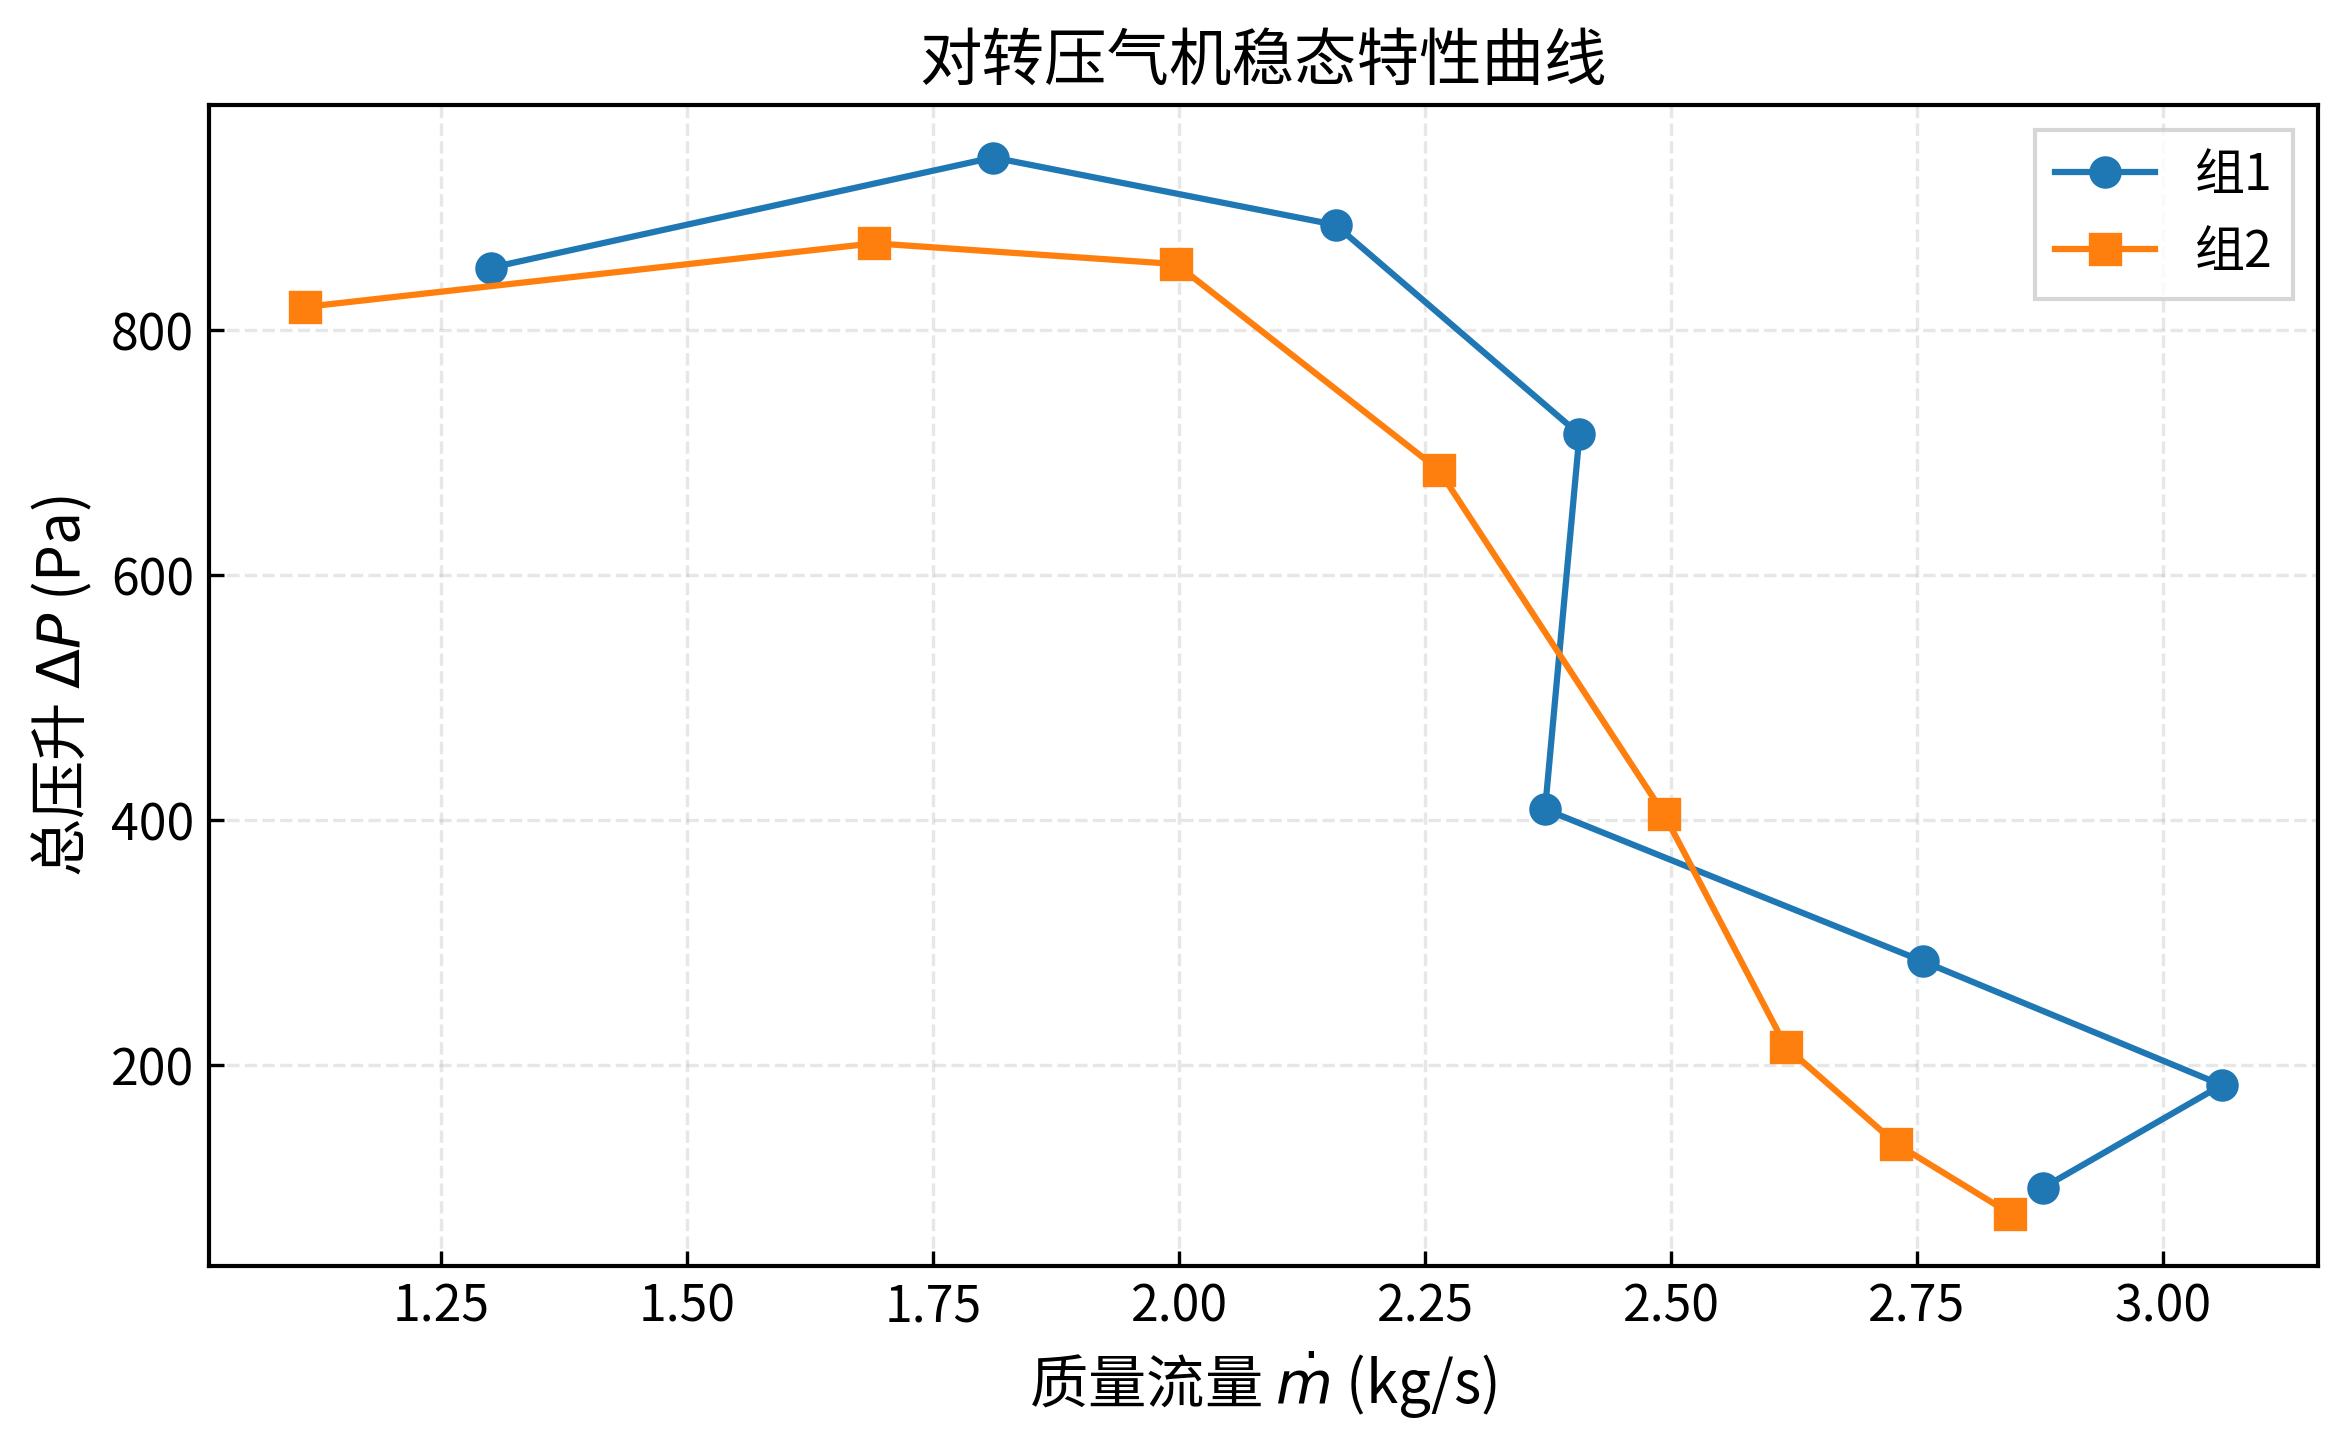
\includegraphics[width=0.90\textwidth]{figures/exp1_2608_characteristics.png}
    \caption{两组转速组合下的对转压气机稳态特性对比}
    \label{fig:2608}
\end{figure}

图~\ref{fig:2608} 给出了两组实验的总压升和总压比随质量流量的变化曲线。

\subsubsection{结果对比分析}

\begin{enumerate}
    \item \textbf{转速组合对总压升的影响}：组1（前1800/后2100 rpm）的最大总压升为941 Pa，组2（前1680/后2220 rpm）为871 Pa。虽然组2的后转子转速更高，但由于前转子转速较低导致进气量减小，整体增压能力低于组1。这表明对转压气机的总性能对前转子的转速更为敏感。

    \item \textbf{节流特性的基本规律}：两组实验中，随着节流角从90° 减小到15°，质量流量均呈下降趋势，总压升随之增大，符合轴流压气机等转速线的典型规律。节流角相同（同为15°）的最后几个工况点之间的差异反映了压气机接近失稳边界时流动状态的不稳定性。

    \item \textbf{失速边界的接近}：当节流角达到15° 时，压气机已接近失稳边界，总压升从最高点开始下降（组1从941降至851 Pa，组2从871降至819 Pa），表明压气机已进入不稳定工作区。此即特性曲线的拐点。

    \item \textbf{叶顶间隙压力特征}：两组实验中上游转子叶顶间隙压力 $P_{\text{ta1}}$ 均高于下游转子 $P_{\text{tb2}}$，反映上游转子对气流的初次加功和下游转子的进一步增压。随着节流角减小，间隙压力均呈上升趋势，与压气机总体增压水平的提高一致。

    \item \textbf{两组对比}：组1（前后转速差较小，30/35 Hz）的总压升普遍高于组2（前后转速差较大，28/37 Hz），说明对转压气机中前后转子的转速合理匹配对性能有重要影响。前后转速比过大或过小均会导致级间流动失配，降低整体效率。
\end{enumerate}

\subsection{思考题}

\begin{enumerate}
    \item \textbf{流量有哪几种计算方法？}\\
    答：常用的流量测量方法包括：
    
    （1）伯努利方程法：通过进口动压（总静压差）计算速度，再乘以密度和流通面积得到质量流量，即本实验采用的方法；
    
    （2）流量管/文丘里管法：利用收缩段前后的静压差，通过标定系数计算流量；
    
    （3）孔板流量计法：利用测量孔板前后的压差计算流量，常用于工业管道；
    
    （4）热线/热膜风速仪法：利用对流换热原理测量局部速度，积分得到流量；
    
    （5）超声波流量计法：利用超声波在流体中的传播时间差计算流量。

    \item \textbf{压比特性线为什么会出现拐点？}\\
    答：压比特性线的拐点反映压气机内部流动状态的转变。在拐点之前，压气机内流动基本稳定，叶片通道内的扩压过程正常进行。拐点之后，叶片吸力面出现大面积附面层分离，流动损失急剧增大，有效增压能力下降。此时压气机进入旋转失速或喘振状态，部分叶片通道内甚至出现回流，导致总压升不再随流量减小而增大，反而下降。拐点的出现位置与叶片负荷水平、来流马赫数、攻角等因素密切相关。

    \item \textbf{简述压力变送器的基本原理。}\\
    答：压力变送器（压力传感器/变送器）将压力信号转换为标准电信号输出。常见原理包括：

    （1）压阻式：利用硅膜片在压力作用下产生弹性变形，导致扩散电阻的电阻值发生变化，通过惠斯通电桥将电阻变化转换为电压信号输出，具有灵敏度高、体积小的特点；
    
    （2）电容式：压力使敏感膜片与固定电极间的距离改变，从而改变电容值；
    
    （3）压电式：利用压电晶体在压力作用下产生电荷，适用于动态压力测量；
    
    （4）应变式：利用金属应变片在弹性元件变形时的电阻变化测量压力。本实验中的压力变送器输出0\textasciitilde5 V或4\textasciitilde20 mA标准信号，经A/D转换后由计算机采集和处理。

    \item \textbf{分析实验中可能出现的误差原因。}\\
    答：误差来源主要包括：
    
    （1）传感器零点漂移：传感器长时间工作后零点偏移，需在实验开始前进行零点采集；
    
    （2）大气条件变化：实验过程中大气温度、压力的波动影响密度和速度的计算；
    
    （3）节流锥定位精度：节流锥位置的手动调节存在读数误差；
    
    （4）气流脉动：压气机进出口气流本身的非定常脉动引起读数波动，需待信号稳定后采集；
    
    （5）数据采集系统A/D转换误差：量化误差和采样精度的影响；
    
    （6）仪器系统误差：压力传感器、大气压力计、温度计等自身精度有限；
    
    （7）温度效应：实验运行过程中电机散热导致进气温度升高，改变空气密度。
\end{enumerate}

\subsection{结论}

通过本次实验，成功测量了低速轴流对转压气机在两组转速下的稳态特性曲线，掌握了压气机气动参数的测量方法和基于伯努利方程的质量流量计算方法。实验结果符合压气机增压的基本理论规律：总压升随转速升高而增大，同一转速下随流量减小而增大。特性曲线的拐点位置和失稳边界的识别为后续压气机稳定性研究提供了实验依据。
